\documentclass[border=4pt, tikz]{standalone}
\usepackage{mathptmx}
\usepackage{amsmath,amssymb}
\usetikzlibrary{arrows.meta,positioning,calc,fit,backgrounds,shapes.geometric,decorations.pathreplacing}

\definecolor{bLin}  {HTML}{CFE2F3}   % linear / convolution
\definecolor{bNorm} {HTML}{FFF2CC}   % normalisation + activation
\definecolor{bSoft} {HTML}{D9EAD3}   % softmax / vector normalisation
\definecolor{bMask} {HTML}{EAD1DC}   % masking
\definecolor{bAgg}  {HTML}{FBD3A8}   % contraction / elementwise product
\definecolor{bPool} {HTML}{E1D5F0}   % pooling
\definecolor{bLoss} {HTML}{F4CCCC}   % objective
\definecolor{bRed}  {HTML}{C0392B}
\definecolor{bInk}  {HTML}{1A1A1A}
\definecolor{bMuted}{HTML}{55606B}
\begin{document}
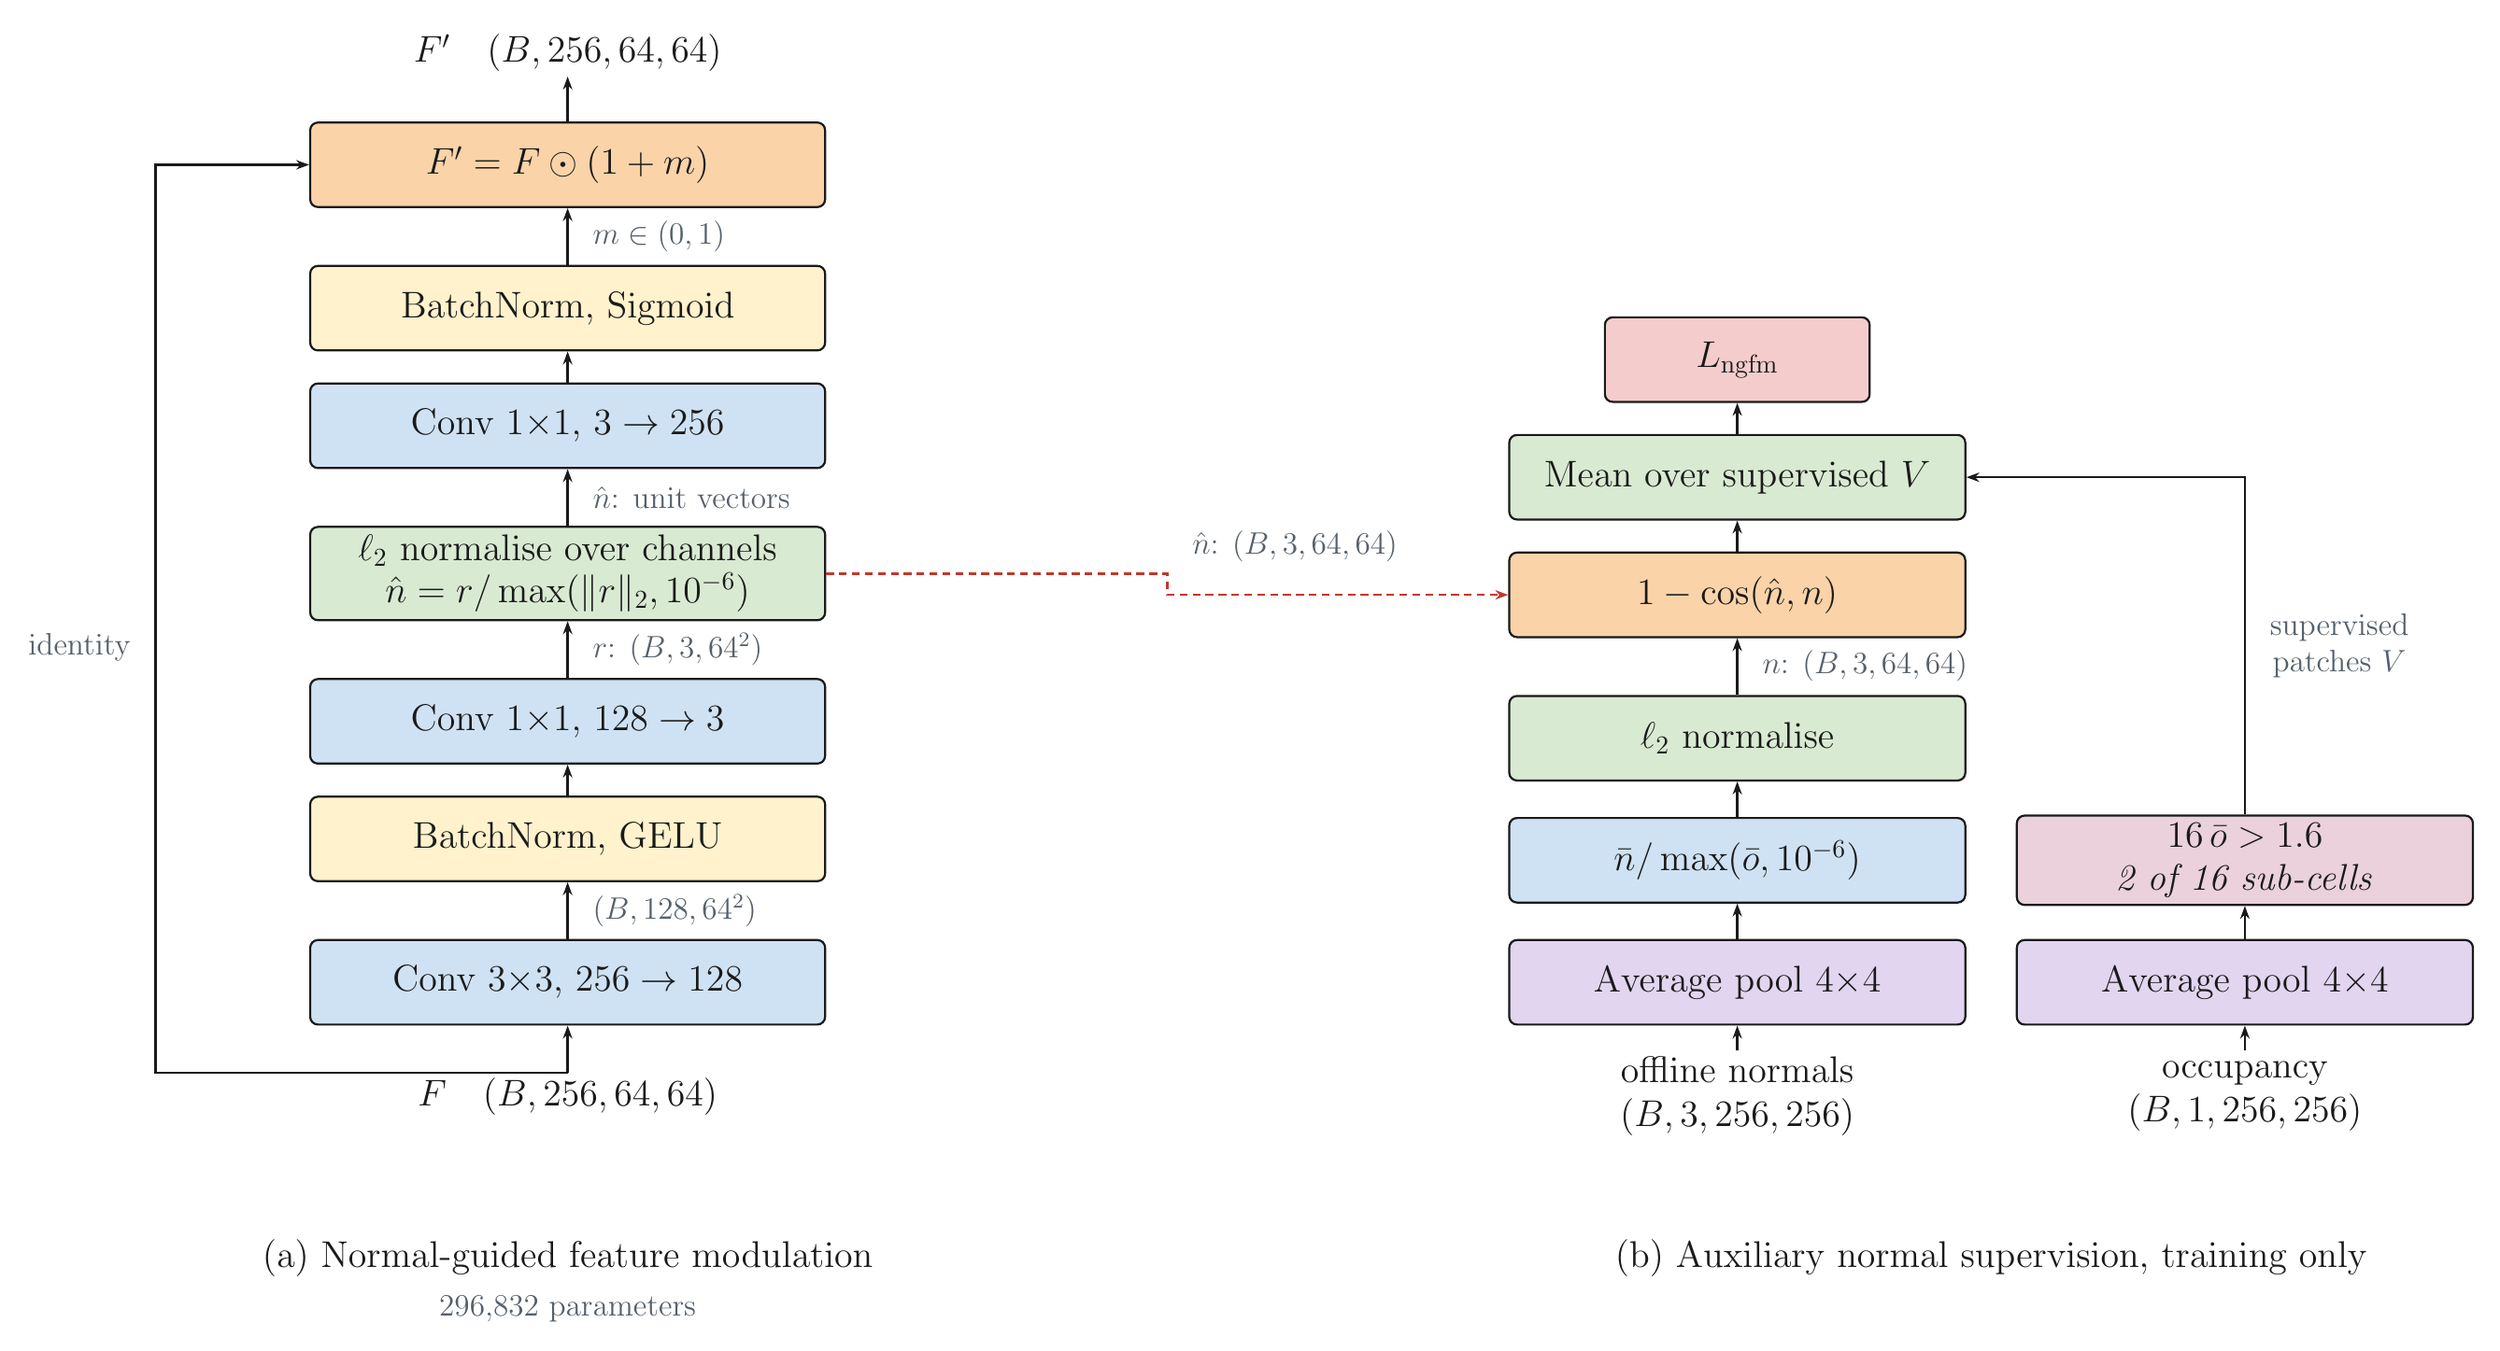
\begin{tikzpicture}[
    blk/.style  ={draw=bInk, line width=0.8pt, rounded corners=3pt, align=center,
                  minimum height=1.15cm, inner xsep=6pt, inner ysep=3pt,
                  text=bInk, font=\fontsize{14}{16.5}\selectfont},
    io/.style   ={align=center, text=bInk, font=\fontsize{14.5}{17}\selectfont},
    % inner sep 1pt so a shape label fits in the gap between two boxes
    shp/.style  ={align=center, text=bMuted, inner sep=1pt,
                  font=\fontsize{12}{14}\selectfont},
    ttl/.style  ={align=center, text=bInk, font=\fontsize{15}{17}\selectfont},
    flow/.style ={-{Stealth[length=5pt,width=3.6pt]}, draw=bInk, line width=0.9pt},
    aux/.style  ={-{Stealth[length=5pt,width=3.6pt]}, draw=bRed, line width=0.9pt,
                  dash pattern=on 3pt off 2pt},
    grp/.style  ={draw=bMuted, line width=0.7pt, dash pattern=on 3pt off 2pt,
                  rounded corners=5pt},
    op/.style   ={draw=bInk, line width=0.8pt, circle, inner sep=1.6pt, fill=white,
                  text=bInk, font=\fontsize{14}{14}\selectfont},
  ]
% ====== panel (a): forward modulation ======
\node[io, anchor=center] at (0.00,0.00) {$F$\quad$(B,256,64,64)$};
\node[blk, fill=bLin, minimum width=7.00cm] (c1) at (0.00,1.55) {Conv $3{\times}3$, $256\to128$};
\node[blk, fill=bNorm, minimum width=7.00cm] (n1) at (0.00,3.50) {BatchNorm, GELU};
\node[blk, fill=bLin, minimum width=7.00cm] (c2) at (0.00,5.10) {Conv $1{\times}1$, $128\to3$};
\node[blk, fill=bSoft, minimum width=7.00cm] (l2) at (0.00,7.11) {$\ell_2$ normalise over channels\\$\hat{n}=r/\max(\Vert r\Vert_2,10^{-6})$};
\node[blk, fill=bLin, minimum width=7.00cm] (c3) at (0.00,9.12) {Conv $1{\times}1$, $3\to256$};
\node[blk, fill=bNorm, minimum width=7.00cm] (n2) at (0.00,10.72) {BatchNorm, Sigmoid};
\node[blk, fill=bAgg, minimum width=7.00cm] (mod) at (0.00,12.67) {$F' = F \odot (1+m)$};
\node[io, anchor=center] at (0.00,14.19) {$F'$\quad$(B,256,64,64)$};
\draw[flow] (0.00,0.32) -- (c1.south);
\draw[flow] (c1) -- (n1);
\draw[flow] (n1) -- (c2);
\draw[flow] (c2) -- (l2);
\draw[flow] (l2) -- (c3);
\draw[flow] (c3) -- (n2);
\draw[flow] (n2) -- (mod);
\draw[flow] (mod.north) -- (0.00,13.87);
\draw[flow] (0.00,0.32) -- (-5.60,0.32) -- (-5.60,12.67) -- (mod.west);
\node[shp, anchor=east] at (-5.90,6.11) {identity};
\node[shp, anchor=west] at (0.30,2.52) {$(B,128,64^2)$};
\node[shp, anchor=west] at (0.30,6.08) {$r$: $(B,3,64^2)$};
\node[shp, anchor=west] at (0.30,8.14) {$\hat{n}$: unit vectors};
\node[shp, anchor=west] at (0.30,11.69) {$m\in(0,1)$};
\node[ttl, anchor=center] at (0.00,-2.20) {(a)~Normal-guided feature modulation};
\node[shp, anchor=center] at (0.00,-2.90) {296{,}832 parameters};
% ====== panel (b): auxiliary supervision, training only ======
\node[io, anchor=center] at (15.90,0.00) {offline normals\\$(B,3,256,256)$};
\node[io, anchor=center] at (22.80,0.00) {occupancy\\$(B,1,256,256)$};
\node[blk, fill=bPool, minimum width=6.20cm] (pn) at (15.90,1.55) {Average pool $4{\times}4$};
\node[blk, fill=bPool, minimum width=6.20cm] (po) at (22.80,1.55) {Average pool $4{\times}4$};
\node[blk, fill=bLin, minimum width=6.20cm] (dv) at (15.90,3.21) {$\bar{n}/\max(\bar{o},10^{-6})$};
\node[blk, fill=bMask, minimum width=6.20cm] (vm) at (22.80,3.21) {$16\,\bar{o} > 1.6$\\\emph{2 of 16 sub-cells}};
\node[blk, fill=bSoft, minimum width=6.20cm] (ln) at (15.90,4.87) {$\ell_2$ normalise};
\node[blk, fill=bAgg, minimum width=6.20cm] (cs) at (15.90,6.82) {$1-\cos(\hat{n},n)$};
\node[blk, fill=bSoft, minimum width=6.20cm] (mm) at (15.90,8.42) {Mean over supervised $V$};
\node[blk, fill=bLoss, minimum width=3.60cm] (ls) at (15.90,10.02) {$L_{\mathrm{ngfm}}$};
\draw[flow] (15.90,0.62) -- (pn.south);
\draw[flow] (22.80,0.62) -- (po.south);
\draw[flow] (pn) -- (dv);
\draw[flow] (dv) -- (ln);
\draw[flow] (ln) -- (cs);
\draw[flow] (cs) -- (mm);
\draw[flow] (mm) -- (ls);
\draw[flow] (po.north) -- (vm.south);
\draw[flow] (22.80,3.84) -- (22.80,8.42) -- (mm.east);
\node[shp, anchor=west] at (23.10,6.13) {supervised\\patches $V$};
\node[shp, anchor=west] at (16.20,5.85) {$n$: $(B,3,64,64)$};
\draw[aux] (l2.east) -- (8.15,7.11) -- (8.15,6.82) -- (cs.west);
\node[shp, anchor=west] at (8.45,7.48) {$\hat{n}$: $(B,3,64,64)$};
\node[ttl, anchor=center] at (19.35,-2.20) {(b)~Auxiliary normal supervision, training only};

\end{tikzpicture}
\end{document}
